%!TEX root = ../main.tex
%%%%%%%%%%%%%%%%%%%%%%%%%%%%%%%%%%
% Links:
%
% Difficulty:
% Companies: 
%%%%%%%%%%%%%%%%%%%%%%%%%%%%%%%%%%

\chapter{Trapping Water}
\label{ch:trapping_water}
\section*{Introduction}
This chapter describes a quite challenging and fun problem that is often asked at big companies like Google and Microsoft. 
In a nutshell the problem asks to find the amount of water that can be trapped in the cavities of a given histogram.


\section{Problem statement}
\begin{exercise}
Given $n$ non-negative integers representing an elevation map (or an histogram) where the width of each bar is $1$, find out how much water it is able to trap after raining.
\end{exercise}


\begin{example}
\label{ex:trapping_water:exmaple1}
	\hfill \\
	\begin{itemize}
		\item[-] Input: $[0,1,0,2,1,0,1,3,2,1,2,1]$
		\item[-] Output: $6$ (See Figure \ref{fig:trapping_water_example1})
	\end{itemize}

	\begin{figure}
		\label{fig:trapping_water_example1}
		\centering
		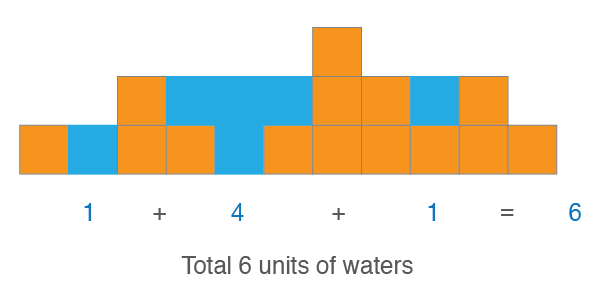
\includegraphics[scale=0.5]{sources/trapping_water/images/example1}
		\caption{Visual representation of the example \ref{ex:trapping_water:exmaple1}}
\end{figure}
\end{example}

\begin{example}
	\hfill \\
	\begin{itemize}
		\item[-] Input: $[1,0,2,1,0,1]  $
		\item[-] Output: $2$
	\end{itemize}
\end{example}

\section{Clarification Questions}

\begin{QandA}
	\item 
	\begin{answered}
		\textit{}
	\end{answered}
	
\end{QandA}

\section{Discussion}
\label{trapping_water:sec:discussion}


\subsection{Brute-force}
\label{trapping_water:sec:bruteforce}
The naive approach consist in for each array element

	\begin{enumerate}
		\item Find the highest bars on left and right sides
		\item add to the final solution the different between the height of the current element minus the minimum between the two hihest bars on left and right
	\end{enumerate}

Why does this work? Because that difference is the amount of water that specific bar can trap.

The complexity of this approach is $O(n^2)$. Finding the maximum elements on left and right costs n, and it needs to be done for all the bars.

\lstinputlisting[language=c++, caption=Sample Caption,label=list:trapping_water]{sources/trapping_water/trapping_water_solution1.cpp}

